%%%% Modèle proposé par kira.ribeiro@universite-paris-saclay.fr %%%%
%%%% màj : 29 octobre 2021 %%%%

\documentclass[english,12pt,a4paper]{book}
\usepackage[utf8]{inputenc}
\usepackage[T1]{fontenc}
\usepackage[english]{babel}
\usepackage[default,oldstyle, scale=.95]{opensans} % police Open Sans
\usepackage{amsmath}
\usepackage{amsfonts}
\usepackage{fancyhdr}
\usepackage{amssymb}
\usepackage{xcolor} % où color selon l'installation
\definecolor{Prune}{RGB}{99,0,60} % l14-33 : couleurs de la charte graphique upsaclay
\definecolor{B1}{RGB}{49,62,72} 
\definecolor{C1}{RGB}{124,135,143}
\definecolor{D1}{RGB}{213,218,223}
\definecolor{A2}{RGB}{198,11,70}
\definecolor{B2}{RGB}{237,20,91}
\definecolor{C2}{RGB}{238,52,35}
\definecolor{D2}{RGB}{243,115,32}
\definecolor{A3}{RGB}{124,42,144}
\definecolor{B3}{RGB}{125,106,175}
\definecolor{C3}{RGB}{198,103,29}
\definecolor{D3}{RGB}{254,188,24}
\definecolor{A4}{RGB}{0,78,125}
\definecolor{B4}{RGB}{14,135,201}
\definecolor{C4}{RGB}{0,148,181}
\definecolor{D4}{RGB}{70,195,210}
\definecolor{A5}{RGB}{0,128,122}
\definecolor{B5}{RGB}{64,183,105}
\definecolor{C5}{RGB}{140,198,62}
\definecolor{D5}{RGB}{213,223,61}
\usepackage{mdframed}
\usepackage{multirow} %% Pour mettre un texte sur plusieurs rangées
\usepackage{multicol} %% Pour mettre un texte sur plusieurs colonnes
\usepackage{tikz}
\usepackage{graphicx}
\usepackage[absolute]{textpos} 
\usepackage{colortbl}
\usepackage{array}
\usepackage{geometry}
\usepackage{titlesec}
\usepackage{hyperref}
\hypersetup{ % paramétrage couleur des liens hypertextes, toujours garder colorlinks=true
    colorlinks=true,
    linkcolor=black,
    urlcolor=purple}


\pagestyle{plain} % pour ne garder que les n°de page en milieu-bas et supprimer les indications de chapitre en marge haute


\usepackage{algorithm}
\usepackage{algpseudocode}

\usepackage{graphicx}
\usepackage{subcaption}
\usepackage{subfiles}

\usepackage{lipsum} % à retirer!!!
\begin{document}

\begin{titlepage}

%\thispagestyle{empty}

\newgeometry{left=6cm,bottom=2cm, top=1cm, right=1cm}

\tikz[remember picture,overlay] \node[opacity=1,inner sep=0pt] at (-13mm,-135mm){
\includegraphics{Frame-ups.pdf}};

%*****************************************************
%******** NUMÉRO D'ORDRE DE LA THÈSE À COMPLÉTER *****
%******** POUR LE SECOND DÉPOT                   *****
%*****************************************************

\color{white}

\begin{picture}(0,0)
\put(-152,-743){\rotatebox{90}{\Large \textsc{THESE DE DOCTORAT}}} \\
\put(-120,-743){\rotatebox{90}{NNT : 2020UPASA001}}
\end{picture}
 
%*****************************************************
%**  LOGO  ÉTABLISSEMENT PARTENAIRE SI COTUTELLE
%**  CHANGER L'IMAGE PAR DÉFAUT **
%*****************************************************
\vspace{-14mm} % à ajuster en fonction de la hauteur du logo
%\flushright 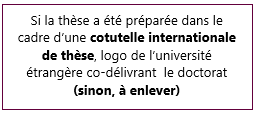
\includegraphics[scale=1]{logo2.png}

%*****************************************************
%******************** TITRE **************************
%*****************************************************

\flushright
\vspace{10mm} % à régler éventuellement
\color{Prune}
\fontfamily{cmss}\fontseries{m}\fontsize{22}{26}\selectfont
  \Huge 

\normalsize
\color{black}
~\\
\Large{Sign Language synthesis by a decreasing granularity system from AZee} \\
\small{\textit{Synthèse de langue des signes par un système d'animation à granularité décroissante à partir d'AZee}} \\
%*****************************************************

\fontfamily{fvs}\fontseries{m}\fontsize{8}{12}\selectfont

\vspace{1.5cm}

\normalsize
\textbf{Thèse de doctorat de l'université Paris-Saclay} \\

\vspace{6mm}

\small École doctorale n°580 : sciences et technologies de l’information et de la communication (STIC)\\
\small Spécialité de doctorat: informatique\\
\small Graduate School : Informatique et sciences du numérique, Référent : Faculté des sciences d’Orsay \\
\vspace{6mm}

\footnotesize Thèse préparée dans l'unité(s) de recherche \textbf{LISN} ((Université Paris-Saclay, CNRS), sous la direction de \textbf{Michael FILHOL}, Directeur de Recherche CNRS \\
\vspace{15mm}

\textbf{Thèse soutenue à Paris-Saclay, le JJ mois AAAA, par}\\
\bigskip
\Large {\color{Prune} \textbf{Paritosh SHARMA}} % Changer le Prénom et le NOM

%************************************
\vspace{\fill} % ALIGNER LE TABLEAU EN BAS DE PAGE
%************************************

\bigskip

\flushleft
\small {\color{Prune} \textbf{Composition du jury}}\\
{\color{Prune} \scriptsize {Membres du jury avec voix délibérative}} \\
\vspace{2mm}
\scriptsize
\begin{tabular}{|p{7cm}l}
\arrayrulecolor{Prune}
\textbf{Prénom NOM} &   Président ou Présidente\\ 
Titre, Affiliation & \\
\textbf{Prénom NOM} &  Rapporteur \& Examinateur / trice \\ 
Titre, Affiliation   &   \\ 
\textbf{Prénom NOM} &  Rapporteur \& Examinateur / trice \\ 
Titre, Affiliation  &   \\ 
\textbf{Prénom NOM} &  Examinateur ou Examinatrice \\ 
Titre, Affiliation   &   \\ 
\textbf{Prénom NOM} &  Examinateur ou Examinatrice \\ 
Titre, Affiliation   &   \\ 
 

\end{tabular} 

\end{titlepage}


% page des résumés à garder en 2ème page. Si les résumés sont trop longs pour tenir sur une seule et même page, on peut mettre un résumé par page
\thispagestyle{empty}
\newgeometry{top=1.5cm, bottom=1.25cm, left=2cm, right=2cm}
\fontfamily{rm}\selectfont

\lhead{}
\rhead{}
\rfoot{}
\cfoot{}
\lfoot{}

\noindent 
%*****************************************************
%***** LOGO DE L'ED À CHANGER IMPÉRATIVEMENT *********
%*****************************************************

\includegraphics[height=2.45cm]{logo_ups_EOBE.png}
\vspace{1cm}
%*****************************************************
\fontfamily{cmss}\fontseries{m}\selectfont

\small

\begin{mdframed}[linecolor=Prune,linewidth=1]

\textbf{Titre:} Synthèse de langue des signes par un système d'animation à granularité décroissante à partir d'AZee

\noindent \textbf{Mots clés:} Animation Graphique, Signeur Virtuel, Langue des Signes

\vspace{-.5cm}
\begin{multicols}{2}
\noindent \textbf{Résumé:}\lipsum[1-2] 
\end{multicols}

\end{mdframed}

\vspace{8mm}

\begin{mdframed}[linecolor=Prune,linewidth=1]

\textbf{Title:} Sign Language Synthesis by a Decreasing Granularity System from AZee

\noindent \textbf{Keywords:} Computer animation, Signing Avatars, Sign Language

\begin{multicols}{2}
\noindent \textbf{Abstract:} \lipsum[1-2]
\end{multicols}
\end{mdframed}

\titleformat{\chapter}[display]
{\normalfont\huge\bfseries\color{black}} % Formatting for chapter title
{\chaptertitlename\ \thechapter} % "Chapter" followed by chapter number
{20pt} % Space between "Chapter" and chapter number
{\Huge} % Formatting for chapter title
[\vspace{2ex}] % Additional space after chapter title

\titlespacing*{\chapter}{0pt}{50pt}{40pt} % Adjusting spacing around chapter title

\titleformat{\section}[hang]{\bfseries\normalsize}{\thesection\ .}{0.5pt}
{\vspace{0.1ex}
}
[\vspace{0.1ex}]
\titlespacing{\section}{1.5pc}{4ex plus .1ex minus .2ex}{.8pc}

\titleformat{\subsection}[hang]{\bfseries\small}{\thesubsection\ .}{1pt}
{\vspace{0.1ex}
}
[\vspace{0.1ex}]
\titlespacing{\subsection}{3pc}{2ex plus .1ex minus .2ex}{.1pc}

\newpage
\thispagestyle{empty}
\vspace*{\fill}
\begin{center}
    \textit{"The only true wisdom is in knowing you know nothing."}\\
    --- \textbf{Socrates}
\end{center}
\vspace*{\fill}
\newpage

\subfile{chapters/acknowledgments/acknowledgments.tex}

\subfile{chapters/resume/resume.tex}

\newgeometry{top=4cm, bottom=4cm, left=2cm, right=2cm}

\newpage
\tableofcontents
\newpage
\listoffigures
\newpage
\listoftables
\newpage

\newgeometry{top=4cm, bottom=4cm, left=4cm, right=4cm}

\subfile{chapters/introduction/introduction.tex}
\subfile{chapters/background_work/background_work.tex}
\subfile{chapters/rigging_layers/rigging_layers.tex}
\subfile{chapters/multi_track/multi_track.tex}
\subfile{chapters/facial_expressions/facial_expressions.tex}
\subfile{chapters/intermediate_blocks/intermediate_blocks.tex}
\subfile{chapters/pose_matching/pose_matching.tex}
\subfile{chapters/conclusion/conclusion.tex}

\newgeometry{top=4cm, bottom=4cm, left=4cm, right=4cm}

\subfile{annex/annex.tex}

\end{document}